\RequirePackage[l2tabu, orthodox]{nag}
\documentclass[french, english]{beamer}
\input{preamble/packages}
\input{preamble/redac}
\input{preamble/math_basics}
%Decision Theory (MCDA and SC)
\NewDocumentCommand{\allalts}{}{\mathcal{A}}
\NewDocumentCommand{\alts}{}{A}
\NewDocumentCommand{\dm}{}{i}
\NewDocumentCommand{\allF}{}{\mathscr{F}}
\NewDocumentCommand{\voters}{}{N}
\NewDocumentCommand{\prof}{}{\boldsymbol{P}}
\NewDocumentCommand{\lprof}{}{\lambda_{\bm{P}}}
%\NewDocumentCommand{\prof}{}{P}
\NewDocumentCommand{\linors}{}{\mathscr{L}(\allalts)}
%Thanks to https://tex.stackexchange.com/q/154549
	%\makeatletter
	%\def\@myRgood@#1#2{\mathrel{R^X_{#2}}}
	%\def\myRgood{\@ifnextchar_{\@myRgood@}{\mathrel{R^X}}}
	%\makeatother
\NewDocumentCommand{\pref}{}{\succ}
\NewDocumentCommand{\prefi}{O{i}}{\succ_{#1}}

\NewDocumentCommand{\PD}{}{\mathit{PD}}
\NewDocumentCommand{\PO}{}{\mathit{PO}}
\NewDocumentCommand{\SPPd}{}{\Sigma^\text{PPd}}
\NewDocumentCommand{\SAll}{}{\Sigma^\text{All}}
\NewDocumentCommand{\SThreshold}{}{\Sigma_\text{threshold}}
\NewDocumentCommand{\vpr}{}{\boldsymbol{v}}

\NewDocumentCommand{\musigma}{O{\sigma}O{P}}{\min_{{#1}\circ\lambda_{{#2}}}(A)}
\NewDocumentCommand{\mustar}{O{\sigma}O{P}}{\min_{{#1} \circ \lambda_{#2}} (\paretopt({#2}))}

\NewDocumentCommand{\alllosses}{}{\intvl{0, m-1}^N}

\NewDocumentCommand{\Ptop}{}{\bar{P}}
\NewDocumentCommand{\sigmatop}{}{\bar{\sigma}}

\NewDocumentCommand{\BK}{O{q}}{\mathit{BK}_{#1}}

%Logic
\NewDocumentCommand{\ltru}{}{\texttt{T}}
\NewDocumentCommand{\lfal}{}{\texttt{F}}


\input{preamble/draw}

%\setbeamertemplate{headline}[singleline]
%\setbeamertemplate{footline}[onlypage]

\title{Ex-ante versus ex-post compromises}
\subject{Social choice}
\keywords{axiomatics, preference aggregation}
\author[B.\ Napolitano, \emph{Olivier Cailloux}, R.\ Sanver]{Beatrice Napolitano \and \emph{Olivier Cailloux} \and Remzi Sanver}
\institute[LAMSADE]{LAMSADE, Université Paris-Dauphine}
\date{\formatdate{24}{11}{2020}}

\begin{document}
\begin{frame}[plain]
	\tikz[remember picture,overlay]{
		\path (current page.south west) node[anchor=south west, inner sep=0] {
			\includegraphics[height=8mm]{Dauphine-Noir.png}
		};
		\path (current page.south east) node[anchor=south east, inner sep=0] {
			\includegraphics[height=1cm]{LAMSADE95.jpg}
		};
		\path (current page.south) ++ (0, 4em) node[anchor=south, inner sep=0] {
			\scriptsize\textcolor{blue}{\url{https://github.com/oliviercailloux/Compromise-pres}}
		};
	}
	\titlepage
\end{frame}
\addtocounter{framenumber}{-1}

\begin{frame}
	\frametitle{Introduction}
		\begin{itemize}
			\item Any reasonable \ac{SCR} reflects an idea of “compromise”
			\item But some arguably less than others (e.\ g.\ plurality)
			\item Let’s investigate the notion of compromise
			\item Several rules explicitly about (some understanding of) compromise
			\item Ours: intuition given by Jean-François Laslier based on the everyday understanding of compromise
			\item Think about a compromise out of a negociation session between political parties
		\end{itemize}
	\begin{block}{The notion of compromise for this talk}
		\begin{itemize}
			\item All individuals
			\item Ex-post
		\end{itemize}
	\end{block}
\end{frame}

\begin{frame}
	\frametitle{Outline}
	\tableofcontents[hideallsubsections, sectionstyle=shaded/show]
\end{frame}

\AtBeginSection{
	\begin{frame}
		\frametitle{Outline}
		\tableofcontents[currentsection, hideallsubsections]
	\end{frame}
}

\section{Ex-post compromises}
\subsection{Introduction}
\begin{frame}
	\frametitle{Context}
	\begin{itemize}
		\item $\voters$ the individuals; $\card{\voters} = n$; $1, 2 \in \voters$
		\item $\allalts$ the alternatives; $\card{\allalts} = m$; $a, b, x, y \in \allalts$
		\item $\linors$, ${\prefi} \in \linors$ a linear order over $\allalts$
		\item $\prof \in \linors^\voters$ a profile
		\item $\powersetz{\allalts}$ the possible winners (the non-empty subsets of $\allalts$)
		\item $f: \linors^\voters → \powersetz{\allalts}$ a \ac{SCR}
	\end{itemize}
	\begin{example}
		\centering
		\begin{tikzpicture}
			\path node (P) {$\prof$};
			\path (P.south) node[anchor=north] (profile) {$%
				\begin{array}{r@{\hspace{1mm} \mapsto \hspace{1mm}}l}
					1 & a \pref_1 b \pref_1 c\\%
					2 & c \pref_2 b \pref_2 a\\%
				\end{array}%
			$};
			\path (profile.east) ++ (3cm, 0) node (f) {$\emptyset ≠ f(\prof) \subseteq \set{a, b, c}$};
		\end{tikzpicture}
	\end{example}
\end{frame}

\begin{frame}
	\frametitle{Our compromises}
	Informally:
	\begin{enumerate}
		\item Determine losses
		\item Determine the most equal losses
		\item Choose some alternatives with most equal losses
	\end{enumerate}
	Formally:
	\begin{enumerate}
		\item Define $\lambda_{\prof}$ that, given $\prof$, obtain loss vectors
		\item Define $\sigma$, an inequality measure over loss vectors
		\item Define two classes of rules using $\sigma$ and $\lambda_{\prof}$
	\end{enumerate}
\end{frame}

\begin{frame}
	\frametitle{Losses}
	\begin{example}[A profile and its loss vectors]
		\centering
		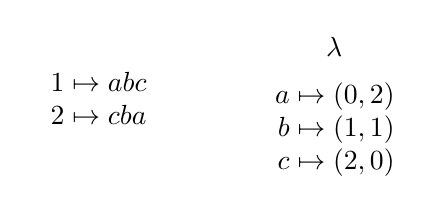
\begin{tikzpicture}
			\path node (P) {$\prof$};
			\path (P.south) node[anchor=north] (profile) {$%
				\begin{array}{r@{\hspace{1mm} \mapsto \hspace{1mm}}l}
					1 & a \pref b \pref c\\%
					2 & c \pref b \pref a\\%
				\end{array}%
			$};
			\path (P.center) ++ (3cm, 0) node (L) {$\lambda_{\prof}$};
			\path (L.south) node[anchor=north] (losses) {$%
				\begin{array}{r@{\hspace{1mm} \mapsto \hspace{1mm}}l}
					a & (0, 2)\\%
					b & (1, 1)\\%
					c & (2, 0)\\%
				\end{array}%
			$};
		\end{tikzpicture}
	\end{example}

	Given $\prof = (\prefi)_{i \in N}$:
	\begin{itemize}
		\item $\lambda_{\prefi}(x) = \card{\set{y \in \allalts \suchthat y \prefi x}} \in \intvl{0, m - 1}$ the loss endured by $i$ when choosing $x \in \allalts$ instead of her favorite alternative
		\item $\lambda_{\prof}: \allalts → \intvl{0, m - 1}^\voters$ s.t. $\lambda_{\prof}(x)$ associates to each voter her loss when choosing $x$
	\end{itemize}
\end{frame}

\begin{frame}
	\frametitle{Inequality}
	\begin{itemize}
		\item We require an inequality measure $\sigma$
		\item Orders completely the loss vectors in $\intvl{0, m - 1}^N$
		\item In order to pick the least unequal loss vectors in $\lambda_{\prof}$
	\end{itemize}
	\begin{block}{Inequality measure}
		\begin{itemize}
			\item $\sigma: \intvl{0, m - 1}^N → \R^+$
			\item $\sigma(l) = 0 ⇔ l = (k)_{i \in N}$ for some $k \in \intvl{0, m - 1}$
			\item $\Sigma$ the set of $\sigma$ satisfying the above
		\end{itemize}
	\end{block}
\end{frame}

\begin{frame}[fragile]
	\frametitle{Minimizing loss vectors}
	Given $\alts \subseteq \allalts$ and $g: \alts → \R$,
	\begin{align}
		\argmin_{x \in \alts}g(x) &= \set{x \in \alts \suchthat g(x) ≤ g(y), \forall y \in \alts}\\
		&= \argmin_\alts g
	\end{align}
	\begin{example}[A profile, its loss vectors and the $\sigma$-minimizer]
		\centering
		\begin{tikzpicture}
			\path node (P) {$\prof$};
			\path (P.south) node[anchor=north] (profile) {$%
				\begin{array}{r@{\hspace{1mm} \mapsto \hspace{1mm}}l}
					1 & a \pref b \pref c\\%
					2 & c \pref b \pref a\\%
				\end{array}%
			$};
			\path (P.center) ++ (3cm, 0) node (L) {$\lambda_{\prof}$};
			\path (L.south) node[anchor=north] (losses) {$%
				\begin{array}{r@{\hspace{1mm} \mapsto \hspace{1mm}}l}
					a & (0, 2)\\%
					b & (1, 1)\\%
					c & (2, 0)\\%
				\end{array}%
			$};
			\path[draw, ->] (P) to (L);
			\path (losses.south) ++ (0, -1cm) coordinate (h2);
			\path ($(P)!.5!(L)$) coordinate (v2);
			\path (h2 -| v2) node (S) {{\visible<1>{\makebox[0pt]{\hspace{3ex}?}}}{\visible<2->{$\set{b}$}}};
			\path[draw, ->] (losses.south) -- (S) node[pos=0.5, anchor=north west, inner sep=0, outer sep=0] {$\argmin_{x \in \allalts} \sigma(\lambda_{\prof}(x))$};
			\onslide<3>{
				\path[draw, ->] (profile.south) -- (S) node[pos=0.5, anchor=north east, inner sep=0, outer sep=0] {$\argmin_{\allalts} (\sigma \circ \lambda_{\prof})$};
			}
		\end{tikzpicture}
	\end{example}
\end{frame}

\subsection{Egalitarian compromises}
\begin{frame}
	\frametitle{Egalitarian compromises}
	An \ac{SCR} is \ac{ECC} iff at each profile, it selects some “minimally inegalitarian” alternative.
	\begin{block}{Egalitarian compromise compatibility}
		An \ac{SCR} $f$ is \ac{ECC} iff 
		\begin{equation}
			\exists \sigma \in \Sigma \suchthat \forall \prof \in \linors^N: f(\prof) \cap \argmin_A (\sigma \circ \lambda_{\prof}) ≠ \emptyset
		\end{equation}
	\end{block}
\end{frame}

\begin{frame}[fragile]
	\frametitle{Paretianism}
	\begin{block}{Paretian rules}
		\begin{itemize}
			\item $\PD(\prof) = \set{x \in \allalts \suchthat \exists y \in \allalts \suchthat y \prefi x, \forall i \in N}$
			\item $\PO(\prof) = \allalts \setminus \PD(\prof)$
			\item An \ac{SCR} $f$ is Paretian iff $\forall \prof \in \linors^N: f(\prof) \subseteq \PO(\prof)$
		\end{itemize}
	\end{block}
	\begin{example}
		$\begin{array}{r@{\hspace{1mm} \mapsto \hspace{1mm}}l}
			1 & a \pref c \pref b \pref d\\%
			2 & c \pref d \pref a \pref b\\%
		\end{array}$%
		\hspace{2cm} $\PD = \only<1>{\text{?}}\onslide<2>{\set{b, d}}$
	\end{example}
\end{frame}

\begin{frame}[fragile]
	\frametitle{Equality and Pareto dominance}
	\ac{ECC} rules are \emph{very} egalitarian
	\begin{example}
		\centering
		\begin{tikzpicture}
			\path node (P) {$\prof$};
			\path (P.south) node[anchor=north] (profile) {$%
				\begin{array}{r@{\hspace{1mm} \mapsto \hspace{1mm}}l}
					1 & a \pref c \pref b\\%
					2 & c \pref a \pref b\\%
				\end{array}%
			$};
			\onslide<2>{
				\path (P.center) ++ (3cm, 0) node (L) {$\lambda_{\prof}$};
				\path (L.south) node[anchor=north] (losses) {$%
					\begin{array}{r@{\hspace{1mm} \mapsto \hspace{1mm}}l}
						a & (0, 1)\\%
						b & (2, 2)\\%
						c & (1, 0)\\%
					\end{array}%
				$};
				\path[draw, ->] (P) to (L);
				\path (losses.south) ++ (0, -1cm) coordinate (h2);
				\path ($(P)!.5!(L)$) coordinate (v2);
				\path (h2 -| v2) node (S) {$\set{b}$};
				\path[draw, ->] (losses.south) -- (S) node[pos=0.5, anchor=north west, inner sep=0, outer sep=0] {$\argmin_{x \in \allalts} \sigma(\lambda_{\prof}(x))$};
				\path[draw, ->] (profile.south) -- (S) node[pos=0.5, anchor=north east, inner sep=0, outer sep=0] {$\argmin_{\allalts} (\sigma \circ \lambda_{\prof})$};
			}
		\end{tikzpicture}
	\end{example}
	\onslide<2>{Egalitarian compromises favor equality over Pareto efficiency}
\end{frame}

\begin{frame}
	\frametitle{ECC $\cap$ Paretian = $\emptyset$}
	I write ECC for the set of \acp{SCR} satisfying ECC, and similarly for other properties
	\begin{theorem}
		ECC $\cap$ Paretian = $\emptyset$ \hfill {\small (for $n, m ≥ 2$)}
	\end{theorem}
	\begin{proof}[Proof (for $m$ = 4; adaptations for any $m ≥ 2$ are straightforward)]
		$\begin{array}{r@{}l@{\hspace{1mm} \mapsto \hspace{1mm}}l}
			1 &\text{ voter} & a_1 \pref a_2 \pref a_3 \pref x\\%
			n - 1 &\text{ voters} & a_2 \pref a_3 \pref a_1 \pref x\\%
		\end{array}$%
		\begin{itemize}
			\item $\forall \sigma \in \Sigma: \argmin_\allalts (\sigma \circ \lambda_{\prof}) = \set{x}$
			\item $f \in \text{ECC} ⇒ x \in f(\prof)$
			\item $f \in \text{Paretian} ⇒ x \notin f(\prof)$ \qedhere
		\end{itemize}
	\end{proof}
\end{frame}

\subsection{Paretian compromises}
\begin{frame}
	\frametitle{Paretian compromises}
	An \ac{SCR} is \ac{PCC} iff at each profile, it selects some “minimally inegalitarian” alternative \emph{among the Pareto optimal ones}.
	\begin{block}{Paretian optimal compatibility}
		An \ac{SCR} $f$ is \ac{PCC} iff 
		\begin{equation}
			\exists \sigma \in \Sigma \suchthat \forall \prof \in \linors^N: f(\prof) \cap \argmin_{\PO(\prof)} (\sigma \circ \lambda_{\prof}) ≠ \emptyset
		\end{equation}
	\end{block}
	Recall:
	\begin{block}{Egalitarian compromise compatibility}
		An \ac{SCR} $f$ is \ac{ECC} iff 
		\begin{equation}
			\exists \sigma \in \Sigma \suchthat \forall \prof \in \linors^N: f(\prof) \cap \argmin_\allalts (\sigma \circ \lambda_{\prof}) ≠ \emptyset
		\end{equation}
	\end{block}
\end{frame}

\subsection{Two remarks}
\begin{frame}
	\frametitle{Paretian compromises and Paretianism}
	PCC does not \emph{require} Paretianism, but is \emph{compatible} with it.
	\begin{itemize}
		\item PCC $\not⇒$ Paretian
		\begin{itemize}
			\item Consider $f(\prof) = \allalts$
			\item $f$ is PCC and $f$ is not Paretian
		\end{itemize}
		\item PCC does not require to select \emph{only} among $\PO(\prof)$
		\item PCC requires to select \emph{some} {(most equal)} alt.\ among $\PO(\prof)$
	\end{itemize}
\end{frame}

%\begin{frame}
%	\frametitle{PCC rules are still very pro-egalitarian}
%	\begin{example}[PCC]
%		$\begin{array}{rl}
%			n - 1 \text{ voters} & a \pref b \pref c\\%
%			1 \text{ voter} & c \pref b \pref a\\%
%		\end{array}$
%		\hspace{2cm} PCC selects? \onslide<2>{$\set{b}$
%	\end{example}
%\end{frame}

\begin{frame}[fragile]
	\frametitle{About our inequality measures}
	Note that $\Sigma$ contains \emph{all} inequality measures that say that constant vectors are the most equal of all.
	\begin{example}[Constraint imposed by PCC]
		\begin{center}
			\begin{tikzpicture}
				\path node (P) {$\prof$};
				\path (P.south) node[anchor=north] (profile) {$%
					\begin{array}{r@{\hspace{1mm} \mapsto \hspace{1mm}}l}
						1 & a \pref b \pref c \pref d\\%
						2 & d \pref a \pref c \pref b\\%
					\end{array}%
				$};
				\onslide<2>{
					\path (P.center) ++ (4cm, 0) node (L) {$\lambda_{\prof}$};
					\path (L.south) node[anchor=north] (losses) {$%
						\begin{array}{r@{\hspace{1mm} \mapsto \hspace{1mm}}l}
							a & (0, 1)\\%
							d & (3, 0)\\%
						\end{array}%
					$};
					\path (losses.south) ++ (0, -1cm) coordinate (h2);
					\path ($(P)!.5!(L)$) coordinate (v2);
					\path (h2 -| v2) node (S) {$\subseteq \set{a, d}$};
					\path[draw, ->] (losses.south) -- (S) node[pos=0.5, anchor=north west, inner sep=0, outer sep=0] {$\argmin_{x \in \PO(\prof)} \sigma(\lambda_{\prof}(x))$};
					\path[draw, ->] (profile.south) -- (S) node[pos=0.5, anchor=north east, inner sep=0, outer sep=0] {$\argmin_{\PO(\prof)} (\sigma \circ \lambda_{\prof})$};
				}
			\end{tikzpicture}
		\end{center}
		\onslide<2>{A PCC $f$ must pick at least one among $a$ and $d$ (depending on $\sigma$)}
	\end{example}
\end{frame}

\section{Comparison}
\subsection{BK compromises}
\begin{frame}
	\frametitle{BK compromise}
	\citet{Brams2001} compromise
	\begin{itemize}
		\item Denoted by $\BK[q]$, with $q \in \intvl{1, n}$
		\item A voter \emph{supports} an alternative at rank $r$ iff she places this alternative at $r$ or better
		\item $\rho_q$: best rank for which some alternative receives $≥ q$ supports
		\item $\BK$ selects the best supported alternatives at rank $\rho_q$
	\end{itemize}
	\begin{example}[{$\BK[3]$}]
		$\begin{array}{r@{\hspace{1mm} \mapsto \hspace{1mm}}l}
			1 & a \pref b \pref c \pref d\\%
			2 & c \pref b \pref a \pref d\\%
			3 & b \pref c \pref d \pref a\\%
			4 & c \pref a \pref d \pref b\\%
			5 & d \pref c \pref b \pref a\\%
		\end{array}$
		\hspace{2cm} $\BK[3]$ selects? \onslide<2>{$\set{c}$ ($\rho_3 = 2$)}
	\end{example}
\end{frame}

\begin{frame}
	\frametitle{Sorts of BK compromises}
	$\BK[\ceil{n / 2}]$ : Majoritarian compromise \citep{Sertel1999} (also “Bucklin” \citep{Erdelyi2015})
	\begin{block}{\citet[abstract]{Sertel1999}}
		\og{}The Majoritarian Compromise is “majoritarian approving” i.e. it always picks “what’s good for a majority” (alternatives which some majority regards as among the better “effective” half of the available alternatives).\fg{}
	\end{block}
	$\BK[n]$: Fallback bargaining
%	\begin{itemize}
%		\item $\rho_n$: the best rank at which some alternative receives unanimous support. $\BK[n]$ selects the best supported alternatives at rank $\rho_n$.
%	\end{itemize}
	\begin{example}[${\BK[n]}$]
		$\begin{array}{rl}
			3 \text{ voters} & a_1 \pref a_2 \pref a_3 \pref a_4\\%
			2 \text{ voters} & a_2 \pref a_1 \pref a_4 \pref a_3\\%
		\end{array}$
		\hspace{2cm} $\BK[n]$ selects? \onslide<2>{$\set{a_1, a_2}$}
	\end{example}
\end{frame}

\begin{frame}
	\frametitle{$\BK, q \in \intvl{1, n}$ is not ECC}
	\begin{theorem}
		$\BK$ is not ECC.\hfill {\small (for $m, n ≥ 2$)}
	\end{theorem}
	\begin{proof}
		$\BK$ is Paretian: consider an alternative $x$ supported by voters $V \subseteq N$ at some rank $r$ and $y \prefi x, \forall i \in V$. Then, the voters in $V$ support $y$ at rank $r$, and never rank $y$ at rank $r$ (as $x$ is at rank $r$ or better). Thus, $V$ supported $y$ already at a better rank. 
		
		The winners in $\BK$ gather $q' ≥ q$ supports at $\rho_q$, and any Pareto-dominating alternative would gather $q' ≥ q$ supports at a better rank. Thus, $\BK$ may not select a Pareto-dominated alternative.
	\end{proof}
\end{frame}

\begin{frame}
	\frametitle{BK compromises (q ≠ n) are not PCC}
	\begin{theorem}
		$\BK, q \in \intvl{1, n - 1}$ is neither ECC nor PCC.\hfill {\small (for $m ≥ 3, n ≥ 2$)}
	\end{theorem}
	\begin{proof}
		$\begin{array}{r@{}l@{\hspace{1mm} \mapsto \hspace{1mm}}l}
			n - 1 &\text{ voters} & x \pref y \pref z \pref …\\%
			1 &\text{ voter} & z \pref y \pref … \pref x\\%
		\end{array}$%
		\begin{itemize}
			\item $\rho_q = 1$ thus $y \notin \BK(\prof)$
			\item $\argmin_{\allalts} (\sigma \circ \lprof) = \set{y}$, thus $f \in ECC ⇒ y \in f(\prof)$
			\item $\argmin_{\PO(\prof)} (\sigma \circ \lprof) = \set{y}$, thus $f \in PCC ⇒ y \in f(\prof)$\qedhere
		\end{itemize}
	\end{proof}
	(This also proves more directly that $\BK, q \in \intvl{1, n - 1}$ fails ECC)
\end{frame}

\begin{frame}
	\frametitle{$\BK[n]$ is PCC}
	Showing that $\BK[n]$ is not PCC requires to restrict $\Sigma$
	\begin{theorem}
		$\BK[n]$ is PCC.
	\end{theorem}
	\begin{proof}[Proof sketch]
		Define $\sigma^\text{discrete}(l) = 1 ⇔ l$ is not constant.
		We prove that $\BK[n] \subseteq \argmin_{\PO(\prof)} (\sigma^\text{discrete} \circ \lprof)$.
		
		If some $x \in \PO(\prof)$ has a constant loss vector, e.\ g.\ $\begin{array}{l}
			a_1 \pref a_2 \pref a_3 \pref a_4 \pref a_5 \pref a_6\\
			a_5 \pref a_4 \pref a_3 \pref a_1 \pref a_2 \pref a_6\\
		\end{array}$, there is exactly one such alternative, $\rho_n$ is its rank, and $\BK[n](\prof) = \set{x}$.

		Otherwise, $\sigma$ does not discriminate among $\PO(\prof)$, thus Paretianism suffices.
	\end{proof}
\end{frame}

\subsection{Condorcet rules}
\begin{frame}
	\frametitle{Condorcet rules}
	$f$ is Condorcet consistent iff $[x \text{ is the Condorcet winner in } \prof ⇒ f(\prof) = \set{x}]$
	\begin{theorem}
		A Condorcet consistent $f$ is neither ECC nor PCC.\hfill {\small (for $m, n ≥ 3$)}
	\end{theorem}
	\begin{proof}
		$\begin{array}{r@{}l@{\hspace{1mm} \mapsto \hspace{1mm}}l}
			n - 1 &\text{ voters} & x \pref y \pref z \pref …\\%
			1 &\text{ voter} & z \pref y \pref … \pref x\\%
		\end{array}$%
		\begin{itemize}
			\item $f$ Condorcet consistent $⇒ f(\prof) = \set{x}$
			\item $f$ ECC $⇒ y \in f(\prof)$
			\item $f$ PCC $⇒ y \in f(\prof)$\qedhere
		\end{itemize}
	\end{proof}
\end{frame}

\subsection{Scoring rules}
\begin{frame}
	\frametitle{Scoring rule}
	\begin{example}[Scoring]
		Given $w = (3, 2, 0)$
		\begin{center}
			\vspace{-3mm}
			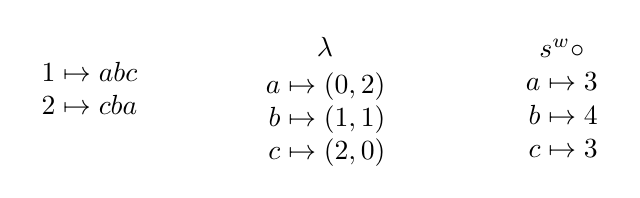
\begin{tikzpicture}
				\path node (P) {$\prof$};
				\path (P.south) node[anchor=north, inner sep=0, outer sep=0] (profile) {$%
					\begin{array}{r@{\hspace{1mm} \mapsto \hspace{1mm}}l}
						1 & a \pref b \pref c\\%
						2 & c \pref b \pref a\\%
					\end{array}%
				$};
				\path (P.center) ++ (3cm, 0) node (L) {$\lambda_{\prof}$};
				\path (L.south) node[anchor=north, inner sep=0, outer sep=0] (losses) {$%
					\begin{array}{r@{\hspace{1mm} \mapsto \hspace{1mm}}l}
						a & (0, 2)\\%
						b & (1, 1)\\%
						c & (2, 0)\\%
					\end{array}%
				$};
				\path (L) ++ (3cm, 0) node (s) {$s^w \circ \lprof$};
				\path (s.south) node[anchor=north, inner sep=0, outer sep=0] (scores) {$%
					\begin{array}{r@{\hspace{1mm} \mapsto \hspace{1mm}}l}
						a & 3\\%
						b & 4\\%
						c & 3\\%
					\end{array}%
				$};
			\end{tikzpicture}
		\end{center}
	\end{example}
	\begin{itemize}
		\item A \emph{weight vector} $w \in \R^{\intvl{0, m - 1}}$ associates a weight to every possible loss
		\item With higher weights for lower losses: $\forall j \in \intvl{0, m - 2}$, $w_j ≥ w_{j + 1}$, and $w_0 ≠ w_{m - 1}$
		\item Score associated to loss vector $(l_k)_{k \in N}$ is $s^w(l) = \sum_{k \in N} w_{l_k}$
		\item $w$ determines the scoring rule $f^w = \argmax_\allalts (s^w \circ \lambda_{\prof})$ that picks those alternatives having highest-scoring loss vectors.
	\end{itemize}
\end{frame}

\begin{frame}
	\frametitle{Scoring rules are not ECC}
	\begin{theorem}
		Consider any weight vector $w$ with $w_j ≥ w_{j + 1}$, and $w_0 ≠ w_{m - 1}$. $f^w$ is not ECC.
		\hfill {\small (for $m, n ≥ 2$)}
	\end{theorem}
	\begin{proof}[Proof (for $m$ = 4; adaptations for any $m ≥ 2$ are straightforward)]
		$\begin{array}{r@{}l@{\hspace{1mm} \mapsto \hspace{1mm}}l}
			1 &\text{ voter} & a_1 \pref a_2 \pref a_3 \pref x\\%
			n - 1 &\text{ voters} & a_2 \pref a_3 \pref a_1 \pref x\\%
		\end{array}$%
		\begin{itemize}
			\item $\argmin_\allalts (\sigma \circ \lambda_{\prof}) = \set{x}$, thus $f \in ECC ⇒ x \in f(\prof)$
			\item $(s \circ \lprof)(x) < (s \circ \lprof)(a_1)$, thus $x \notin f^w(\prof)$ \qedhere
		\end{itemize}
	\end{proof}
\end{frame}

\begin{frame}
	\frametitle{Anti-plurality}
	\begin{itemize}
		\item $w$ is an Anti-plurality (AP) weight vector iff $w_0 = w_{m - 2}$.
		\item Example: $w = (3, 3, 3, 0)$
	\end{itemize}
	\begin{theorem}
		Given an AP $w$, $f^w$ is PCC \hfill {\small (for $m ≥ 2$)}
	\end{theorem}
	\begin{proof}[Proof idea]
		Define $\sigma^\text{discrete}(l) = 1 ⇔ l$ is not constant.
		To prove: $\exists x \in f^w(\prof) \cap \argmin_{\PO(\prof)} (\sigma^\text{discrete} \circ \lprof)$.
		
		Assume $\prof$ contains some $x \in \PO(\prof)$ with a constant loss vector, e.\ g.\ 
		$\begin{array}{l}
			a_1 \pref a_2 \pref a_3 \pref a_4\\
			a_3 \pref a_2 \pref a_1 \pref a_4\\
		\end{array}$.
		This $x$ is never last, so $x \in f^w(\prof)$.
		
		Otherwise, $\sigma$ does not discriminate among $\PO(\prof)$. Take any $x \in \PO(\prof) \cap f^w$.
	\end{proof}
\end{frame}

\begin{frame}
	\frametitle{Scoring rules not AP are not PCC for large enough $n$}
	\begin{theorem}
		Given a non AP $w$, $m ≥ 3$ and a large enough $n$, $f^w$ is not PCC.
	\end{theorem}
	\begin{proof}[Sketch of proof]
		$\begin{array}{rl}
			i = 1 & a_2 \pref … \pref a_m \pref a_1\\%
			2 ≤ i ≤ m - 2 & a_1 \pref … \pref a_m \pref a_i\\%
			m - 1 ≤ i ≤ n & a_1 \pref … \pref a_m \pref a_{m - 1}\\%
		\end{array}$%
		\begin{itemize}
			\item $\argmin_{\PO(\prof)} (\sigma \circ \lprof) = \set{a_m}$, thus $f \in PCC ⇒ a_m \in f(\prof)$
			\item For $n$ large enough, $(s \circ \lprof)(a_1) > (s \circ \lprof)(a_m)$, thus $a_m \notin f^w(\prof)$ \qedhere
		\end{itemize}
	\end{proof}
	We see that PCC rules are \emph{very} egalitarian
\end{frame}

\subsection{Restricting \texorpdfstring{$\Sigma$}{Sigma}}
\begin{frame}
	\frametitle{Restricting $\Sigma$}
	\begin{itemize}
		\item Among the rules seen here, only $\BK[n]$ and Anti-plurality are PCC
		\item Proved using a “weird” $\sigma$ inequality measure
		\item This positive result vanishes with a slight supplementary restriction on $\Sigma$
	\end{itemize}
	\begin{definition}[Condition $C_{m, n}$]
		Given $m ≥ 4, n ≥ \max\set{4, m - 1}$, $\sigma$ satisfies condition $C_{m, n}$ iff $\sigma(m - 3, m - 1, m - 2, …, m - 2) < \sigma(m - 2, m - 3, …, 1, 0, …, 0)$.
	\end{definition}
	\begin{example}%[Examples of conditions $C$]
		$C_{5, 4}$ requires $\sigma(2, 4, 3, 3) < \sigma(3, 2, 1, 0)$.

		$C_{6, 5}$ requires $\sigma(3, 5, 4, 4, 4) < \sigma(4, 3, 2, 1, 0)$.
	\end{example}
\end{frame}

\begin{frame}
	\frametitle{Under condition \texorpdfstring{$C_{m, n}$}{C(m, n)}}
	\begin{theorem}
		Under condition $C_{m, n}$, and  given an AP $w$, $\BK[n]$ and $f^w$ $\notin$ PCC.
	\end{theorem}
	\begin{proof}[Proof for $m = 5, n = 4$]
		$\begin{array}{r@{\hspace{1mm} \mapsto \hspace{1mm}}lllll}
			1 &	&	&x	&y	&a_1\\%
			2 &	&	&y	&	&x\\%
			3 &	&y	&	&x	&a_2\\%
			4 &y	&	&	&x	&a_3\\%
		\end{array}$%
		\begin{itemize}
			\item $y$ is the only alt.\ never last, thus for both rules: $f(\prof) = \set{y}$
			\item $\lprof(x) = (2, 4, 3, 3)$, $\lprof(y) = (3, 2, 1, 0)$ thus $(\sigma \circ \lprof)(x) < (\sigma \circ \lprof)(y)$
			\item and $x \in \PO(\prof)$, thus $y \notin \argmin_{\PO(\prof)}(\sigma \circ \lprof)$ \qedhere
		\end{itemize}
	\end{proof}
	We see (again) that PCC rules are \emph{very} egalitarian
\end{frame}

\section{Two individuals}
\subsection{\texorpdfstring{$\BK[n = 2]$}{BK for two individuals}}
\begin{frame}
	\frametitle{Bargaining contexts}
	\begin{itemize}
		\item We see that our compromise rules place an important emphasis on equality
		\item This might be particularly justified in bargaining contexts
		\item Appears comparatively harder to justify in voting contexts
		\item \citet{Brams2001} indicate that they recommend the rule $\BK[n]$ particularly in bargaining contexts
		\item Let’s see how $\BK[n = 2]$ relate to PCC
	\end{itemize}
\end{frame}

\begin{frame}
	\frametitle{Restricting $\Sigma$ for two individuals}
	Showing that $\BK[n = 2]$ is not PCC requires to restrict $\Sigma$
	\begin{definition}[Condition $D_m$]
		Given $m ≥ 7$ odd, $\sigma$ satisfies condition $D_m$ iff $\sigma(\frac{m - 1}{2} + 1, \frac{m - 1}{2} - 1) < \sigma(0, \frac{m - 1}{2})$
	\end{definition}
	\begin{example}
		$D_7$ requires $\sigma(4, 2) < \sigma(0, 3)$

		$D_9$ requires $\sigma(5, 3) < \sigma(0, 4)$
	\end{example}
\end{frame}

\begin{frame}
	\frametitle{$\BK[n = 2]$ is not PCC under condition $D$}
	\label{sl:bknnotpcc}
	\begin{theorem}
		Given $m ≥ 7$ odd and $n = 2$, under condition $D_m$, $\BK[n]$ is not PCC.
	\end{theorem}
	\begin{proof}[Proof \hfill {\small [illustrations for $m = 9$]}]
		Define $\alpha = \frac{m - 1}{2}$, $\beta = \frac{m - 1}{2} - 1$ \hfill {\small [$\alpha = 4, \beta = 3$]}

		$\begin{array}{r@{\hspace{1mm} \mapsto \hspace{1mm}}lllllllll}
			1 & x &\pref a_1 &\pref a_2 &\pref … &\pref a_\alpha &\pref y &\pref b_1 &\pref … &\pref b_\beta\\
			2 & b_1 &\pref … &\pref b_\beta &\pref y &\pref x &\pref a_1 &\pref a_2 &\pref … &\pref a_\alpha\\
		\end{array}$%
		\begin{itemize} 
			\item $\BK[n] = \set{x}$
			\item $\lprof(y) = (\alpha + 1, \beta)$, $\lprof(x) = (0, \beta + 1)$ thus $(\sigma \circ \lprof)(y) < (\sigma \circ \lprof)(x)$ \hfill {\small [$\lprof(y) = (5, 3)$, $\lprof(x) = (0, 4)$]}
			\item and $y \in \PO(\prof)$, thus $x \notin \argmin_{\PO(\prof)}(\sigma \circ \lprof)$ \qedhere
		\end{itemize}
	\end{proof}
\end{frame}

\subsection{Other rules}
\begin{frame}
	\frametitle{Other two person bargaining rules}
	Similar results hold for: 
	\begin{itemize}
		\item $\BK[n]$, $m$ even
		\item Pareto-and-Veto rules \citep{Laslier2020}
		\item Veto-Rank mechanism \citep{Clippel2014}
		\item Shortlisting \citep{Clippel2014}
	\end{itemize}
	The proofs are very similar to the one just shown.
\end{frame}

\subsection{Discussion}
\begin{frame}
	\frametitle{Discussion}
	\begin{itemize}
		\item Our compromises try to make everybody concede equally
		\item Disagree with many rules
		\item Might be considered too egalitarian, but (I’d argue) interesting to study conceptually
		\item Might lead to question Pareto in favor of equality (already studied?)
		\item Possibly fitting some bargaining behavior (think about ultimatum games)
	\end{itemize}
\end{frame}

\begin{frame}[plain]
	\addtocounter{framenumber}{-1}
	\begin{center}
		\huge
		\textit{Thank you for your attention!}
	\end{center}
\end{frame}

\appendix
\AtBeginSection{
}
%- Appendix: I put a before b from my own perspective; but considering 1’s POV, I prefer b to a: either because I am envious, or even one could say that my objective interest is that b > a, even when I ignore that a is there. When my pref chg because of someone else, it is considered envy, but it may be about my interest.
%- Not ashamed of this very egalitarian focus but we’re willing to compromise to cope with classical demands of our fellow economist colleagues.

\section{Plurality}
\begin{frame}
	\frametitle{Plurality}
	Plurality selects the alternatives most often at first rank
	\begin{example}[Plurality]
		$\begin{array}{r@{\hspace{1mm} \mapsto \hspace{1mm}}l}
			1 & a \pref b \pref c \pref d\\%
			2 & a \pref b \pref c \pref d\\%
			3 & b \pref c \pref d \pref a\\%
			4 & c \pref b \pref d \pref a\\%
			5 & d \pref b \pref c \pref a\\%
		\end{array}$
		\hspace{2cm} Plurality selects? \onslide<2>{$\set{a}$}
		
		\vspace{1em}
		Here, Plurality only “considers” a minority of individuals.
	\end{example}
\end{frame}

\section{Ex-ante compromises}
\begin{frame}
	\frametitle{A compromise may be exclusively ex-ante}
	\begin{example}[{$\BK[51]$}]
		$\begin{array}{rl}
			49\text{ voters} & a \pref b \pref c\\%
			51\text{ voters} & c \pref b \pref a\\%
		\end{array}$
		\hspace{2cm} $\BK[51]$ selects? \onslide<2>{$\set{c}$ ($\rho_{51} = 1$)}
	\end{example}
	\begin{itemize}
		\item Actually \emph{nobody} conceded anything here
		\item “Ex-ante” compromise: a priori willingness to compromise may not require compromising
		\item Observation holds for any $q \in \intvl{1, n - 1}$
		\item See Slide \ref{sl:bknnotpcc} for an application to the case $q = n$
	\end{itemize}
\end{frame}

%\clearpage\pdfbookmark[2]{\refname}{\refname}
\begin{frame}[allowframebreaks]
	\frametitle{\refname}
 	\bibliography{biblio}
\end{frame}

\clearpage\pdfbookmark[2]{License}{License}
\begin{frame}[plain]
	\frametitle{License}
	This presentation, and the associated \LaTeX{} code, are published under the \href{https://opensource.org/licenses/MIT}{MIT license}. Feel free to reuse (parts of) the presentation, under condition that you cite the author.
	
	Credits are to be given to \hrefblue{https://www.lamsade.dauphine.fr/~ocailloux/}{Olivier Cailloux}, Université Paris-Dauphine.
\end{frame}
\addtocounter{framenumber}{-1}
\end{document}

\begin{frame}
	\frametitle{Title}
	\begin{block}{Block}
%		\setlength\abovedisplayskip{1 ex}% reduce space above equations
		\begin{itemize}
			\item Item
		\end{itemize}
	\end{block}
	\begin{itemize}
		\item Item
	\end{itemize}
\end{frame}

